\documentclass{article}
\usepackage{amsmath}
\usepackage{graphicx}
\usepackage{booktabs}

\title{Comprehensive Test}
\author{Test Author}
\date{\today}

\begin{document}

\maketitle

\section{Text Basics}

Hello   World!   Multiple   spaces   collapsed.
中文测试。你好世界！

%中英文混合测试
Mixed English      and     中文   with   extra   spaces.
中I文and与you英文间 can 需要添加的空after 格，的确是这样的 Can，不能不UFO加空格，above     不然影响美观。
天、    blue ， good地。 yes or    ，no问题
Paragraph one.
\textbf{Bold text} and \textit{italic} and \emph{emphasis}.

%中文与公式混合测试
天地人，$\beta$、是月星 $A$是 $B$要地  $n$  同    $\int$ 口$\beta$   一要。$m$、$5$，是的$1$ ！   $j$是



Paragraph two after blank lines.
Text % line-end comment
% Standalone comment
More text

\section{Inline Math}
The equation $E = mc^2$ is famous.

Using \( \sum_{i=1}^{n} i \) inline.

The variable $x$ and constant $\pi$.

\section{Display Math}

\[
\int_0^1 f(x) \, dx
\]





%公式测试
公式 $$ \lim_{n \to \infty} \frac{1}{n} = 0 $$可以看一下    $$\beta+\alpha$$这个$$ \lim_{n \to \infty} \frac{1}{n} = 0 $$




\section{Equations}

\begin{equation}
E = mc^2
\end{equation}

\begin{equation*}
\nabla \cdot \mathbf{E} = \frac{\rho}{\epsilon_0}
\end{equation*}

\section{Alignment}

\begin{align}
x & = 1 & y & = 2 \\
z & = 3 & w & = 4
\end{align}

\begin{align*}
f(x) & = x^2 + 2x + 1 \\
     & = (x+1)^2
\end{align*}

\section{Command Shorthand}

\frac12 should become \frac{1}{2}.

 $\frac34$ also works.

\sqrt{x} and \sqrt[3]{x}.

\section{Tables}

\begin{table}[h]
\centering
\begin{tabular}{lcc}
\toprule
Name & Value & Unit \\
\midrule
Alpha & 1.23 & m \\
Beta & 4.56 & s \\
\bottomrule
\end{tabular}
\caption{Sample table}
\label{tab:sample}
\end{table}

\section{Lists}

\begin{itemize}
\item First item
\item Second item with \textbf{bold}
\item Third item
\end{itemize}

\begin{enumerate}
\item Numbered one
\item Numbered two
\end{enumerate}

\section{Verbatim}

\begin{verbatim}
Do not \format this % comment
\frac{1}{2} stays as is
\end{verbatim}

Also \verb|skip this| and \verb!delim!.

\section{Figures}

\begin{figure}[h]
\centering
\fbox{Placeholder image}
\caption{Sample figure}
\label{fig:sample}
\end{figure}

\section{Cross References}

See Table~\ref{tab:sample} and Figure~\ref{fig:sample}.

\section{Nested Math}

\begin{equation}
\begin{pmatrix}
a & b \\
c & d
\end{pmatrix}
\begin{pmatrix}
e \\
f
\end{pmatrix}
=
\begin{pmatrix}
ae + bf \\
ce + df
\end{pmatrix}
\end{equation}

\section{Error Recovery}

This has an unmatched } brace.

\frac{1}{2} after the error.

\section{Custom Commands}

\newcommand{\R}{\mathbb{R}}

The set $\R$ and norm.

\section{TikZ}

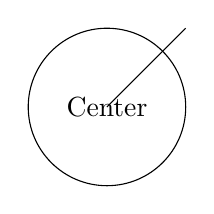
\begin{tikzpicture}
\draw (0,0) circle (1);
\draw (0,0) -- (1,1);
\node at (0,0) {Center};
\end{tikzpicture}

\section{Deep Nesting}

\begin{itemize}
\item Level 1
\begin{itemize}
\item Level 2
\begin{itemize}
\item Level 3
\end{itemize}
\end{itemize}
\end{itemize}

\section{Mixed Content}




Some text $x = 1$ and % inline math with comment
more text.

% Multiple
% consecutive
% comments

Final paragraph.

\end{document}
